\subsection{三档画质与本次实测带宽}
Q60、Q75、Q85 是本工程 JPEG 量化表的质量档位。较高 Q 通常保留更多量化后的细节，并增加 JPEG 大小；Q 值本身不是百分比压缩率。实际压缩比必须由原始有效载荷与压缩后的字节数计算，并注明原始格式。

本次在同一实验室场景、N32、彩色模式下依次测量三档画质，末尾再次测量 Q60，检查分时采集的场景漂移。每档切换后确认状态读回并等待稳定，采样约 12 s。下表使用十进制单位 $1\,\mathrm{kB}=1000$ B、$1\,\mathrm{MB}=10^6$ B；界面单帧大小使用 KiB，$1\,\mathrm{KiB}=1024$ B。

\begin{table}[H]\centering\caption{同场景 JPEG 质量与带宽实测}\label{tab:livequality}
\small\begin{tabular}{@{}lrrrrr@{}}\toprule
画质 & 样本帧数 & 均值 (kB/帧) & JPEG (MB/s) & USB (MB/s) & 压缩比\\\midrule
Q60 & 362 & 172.45 & 5.175 & 5.238 & 24.05:1\\
Q75 & 361 & 239.68 & 7.182 & 7.269 & 17.30:1\\
Q85 & 364 & 339.34 & 10.203 & 10.325 & 12.22:1\\
Q60 复测 & 363 & 172.27 & 5.178 & 5.241 & 24.07:1\\
\bottomrule\end{tabular}\end{table}

\begin{figure}[H]\centering
\begin{tikzpicture}
\begin{axis}[width=.88\linewidth,height=5.8cm,ybar,bar width=14pt,
 ymin=0,ylabel={带宽 (MB/s)},symbolic x coords={Q60,Q75,Q85},xtick=data,
 ymajorgrids=true,grid style={gray!20},legend style={at={(0.5,1.03)},anchor=south,legend columns=2,draw=none,column sep=8pt},
 legend image code/.code={\draw[#1] (0cm,-.1cm) rectangle (.28cm,.1cm);},
 enlarge x limits=.23]
\addplot[fill=teal!65,draw=teal] coordinates {(Q60,5.175) (Q75,7.182) (Q85,10.203)};
\addplot[fill=gray!45,draw=gray] coordinates {(Q60,5.238) (Q75,7.269) (Q85,10.325)};
\legend{JPEG 有效载荷,USB 接收记录}
\end{axis}\end{tikzpicture}
\caption{本次实测质量档位与带宽关系。帧率均约 30 fps，USB 读出记录包含 MBLK 开销。}\label{fig:livebandwidth}
\end{figure}
本次场景中，从 Q85 调低至 Q60，JPEG 平均载荷率从 10.203 MB/s 降至 5.175 MB/s，减少约 49.3\%。末尾 Q60 复测为 5.178 MB/s，相对首次变化 +0.04\%，用于提示分时统计的波动范围；不作为同输入压缩的严格误差界限。
\clearpage
\subsection{Q60 与 Q75 的界面带宽对照}
\begin{figure}[H]\centering
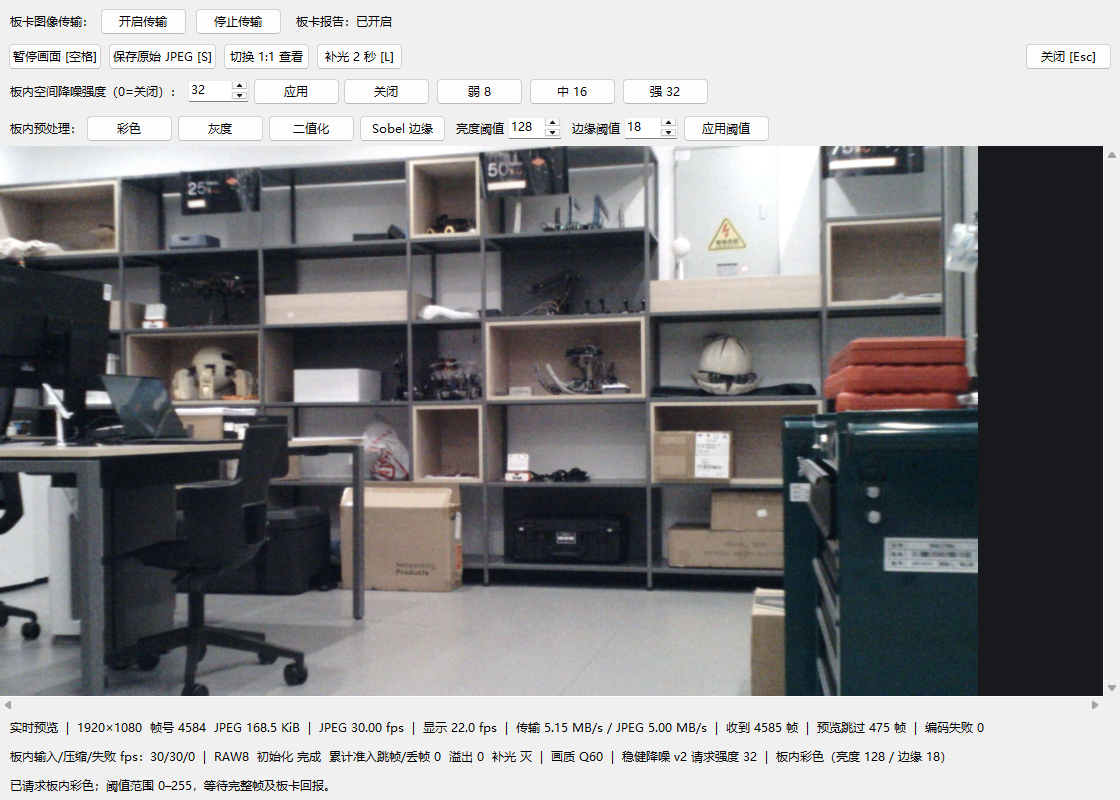
\includegraphics[width=.82\linewidth]{quality_q60_window.png}
\caption{彩色 Q60，N32。较低质量档位减少本场景的编码字节数。截图时 JPEG 168.5 KiB；稳定窗口 JPEG 载荷 5.18 MB/s、USB 接收 5.24 MB/s。}\label{fig:quality60}
\end{figure}
\begin{figure}[H]\centering
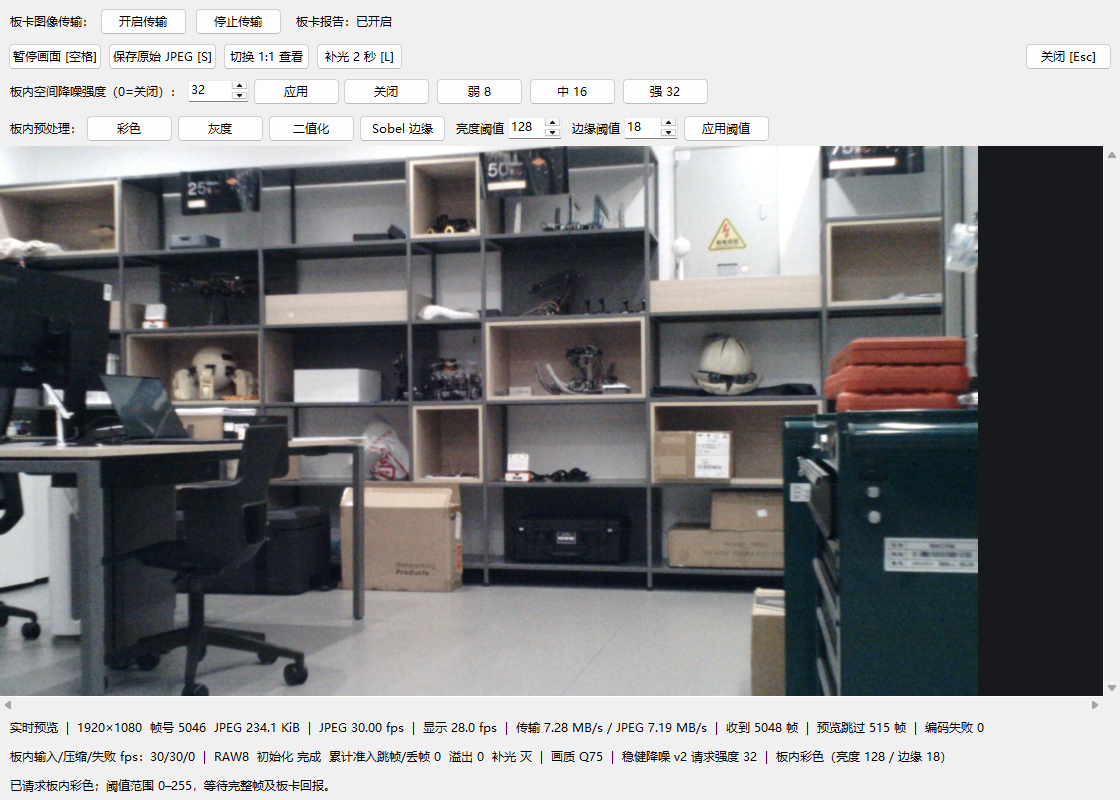
\includegraphics[width=.82\linewidth]{quality_q75_window.png}
\caption{彩色 Q75，N32。底部状态同时显示质量、帧大小、帧率和传输带宽。截图时 JPEG 234.1 KiB；稳定窗口 JPEG 载荷 7.18 MB/s、USB 接收 7.27 MB/s。}\label{fig:quality75}
\end{figure}
\clearpage
\subsection{Q85 与 Q60 复测的界面对照}
\begin{figure}[H]\centering
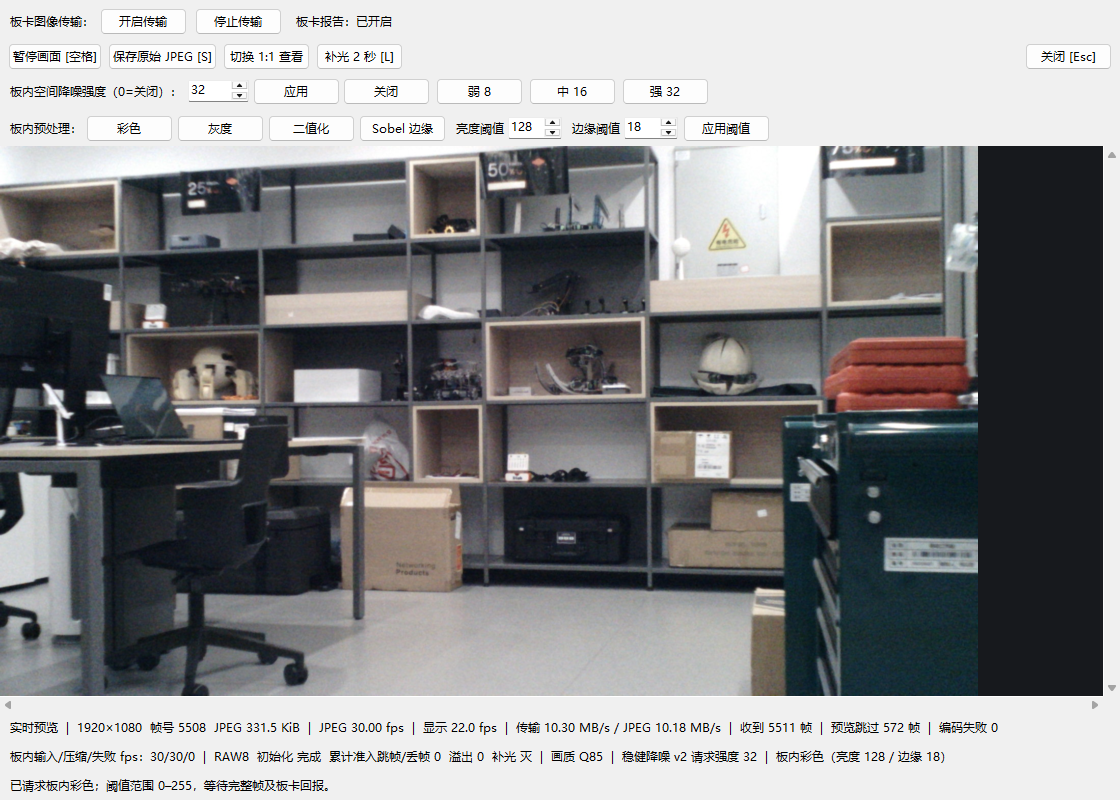
\includegraphics[width=.82\linewidth]{quality_q85_window.png}
\caption{彩色 Q85，N32。本次场景中载荷高于 Q60 和 Q75。截图时 JPEG 331.5 KiB；稳定窗口 JPEG 载荷 10.20 MB/s、USB 接收 10.32 MB/s。}\label{fig:quality85}
\end{figure}
\begin{figure}[H]\centering
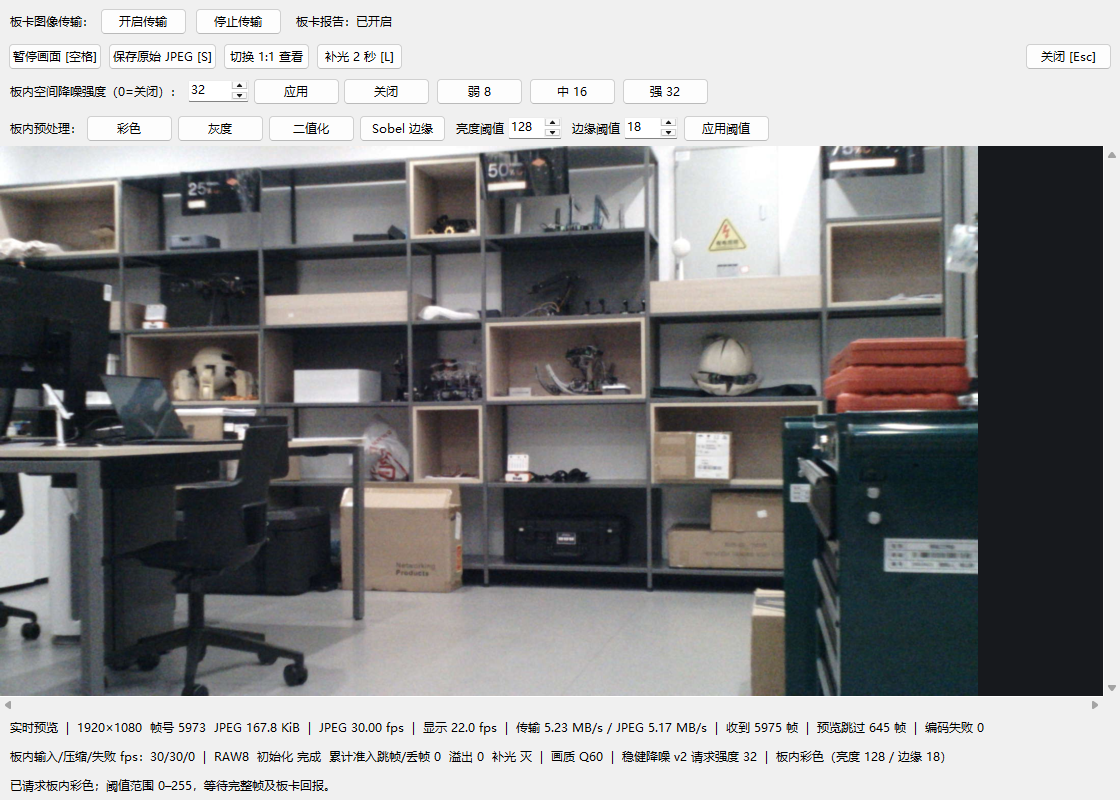
\includegraphics[width=.82\linewidth]{quality_q60_repeat_window.png}
\caption{返回彩色 Q60 复测，N32。检查本次分时采集的载荷漂移。截图时 JPEG 167.8 KiB；稳定窗口 JPEG 载荷 5.18 MB/s、USB 接收 5.24 MB/s。}\label{fig:quality60-repeat}
\end{figure}
\clearpage
\subsection{压缩比与带宽口径}
以编码前 YUV422 有效像素为参照，一帧大小为
\[
 S_{\rm YUV422}=1920\times1080\times2=4\,147\,200\ \mathrm{B},\qquad
 B_{\rm raw,30}=124.416\ \mathrm{MB/s}.
\]
设稳定窗口平均 JPEG 大小为 $\overline S_{\rm JPEG}$，则
\[
 R=\frac{4\,147\,200}{\overline S_{\rm JPEG}},\qquad
 \eta=\left(1-\frac{\overline S_{\rm JPEG}}{4\,147\,200}\right)\times100\%,\qquad
 B_{\rm JPEG}\approx\overline S_{\rm JPEG}\,f/10^6.
\]
Q60 的平均 JPEG 为 172445.76 B，按 YUV422 计算压缩比 24.05:1，有效载荷减少 95.84\%。Q75 的平均 JPEG 为 239675.46 B，按 YUV422 计算压缩比 17.30:1，有效载荷减少 94.22\%。Q85 的平均 JPEG 为 339341.77 B，按 YUV422 计算压缩比 12.22:1，有效载荷减少 91.82\%。

若改用传感器 RAW8 作为参照，一帧为 $2\,073\,600$ B，相应压缩比减半；两种基准不可混写。表\ref{tab:livequality}统一采用 YUV422。当前灰度、二值化和边缘仍沿用 JPEG 颜色帧及中性色度的链路格式，视觉上单色并不意味着传输变成无损 1 bit 像素流。

统计中的 JPEG 带宽为接收的完整 JPEG 字节增量除以主机单调时钟间隔；USB 带宽为相同窗口内解析器收到的 MBLK 记录字节增量，包含分块头、帧描述和状态记录。它不包含 USB 物理层握手、总线填充等全部开销，所以不能直接等同于 USB 总线利用率，也不能用标称 USB 2.0 速率直接反推链路余量。

本次 16 个稳定窗口的编码失败、FIFO 溢出及板内准入跳帧/丢帧增量均为 0，板卡时间戳计算的帧率约为 30.0019 fps。GUI 只解码显示选中的最新帧，本次采集未声明每个接收帧都经过独立完整像素解码；逐帧完整解码验收由前述严格接收器历史测试提供。截图不能单独替代长时间稳定性测试。
\evid{evidence/quality_q60.json；quality_q75.json；quality_q85.json；quality_q60_repeat.json}
\clearpage
